\chapter{分类与逻辑回归}

现在我们转向分类问题。这与回归问题类似,主要区别在于需要预测的目标变量 $y$ 只能取有限的离散值。目前,我们将重点讨论二元分类 (binary classification) 问题,其中 $y$ 的取值仅限于 0 和 1。(这里讨论的大部分内容也适用于多类别分类情况。)例如,在构建垃圾邮件分类器时,$x^{(i)}$ 可以代表一封电子邮件的某些特征,而 $y$ 则表示该邮件是否为垃圾邮件(垃圾邮件为 1,非垃圾邮件为 0)。通常,0 被称为\textbf{负类 (negetive class)},1 被称为\textbf{正类 (positive class)},有时也用符号 “$-$” 和 “$+$” 表示。对于给定的输入特征 $x^{(i)}$,其对应的 $y^{(i)}$ 被称为该训练样本的\textbf{标签 (label)}。

\section{逻辑回归}\label{sec:2.1}

在处理分类问题时,我们可以暂时忽略目标变量 $y$ 是离散值这一特性,并沿用之前的线性回归算法来尝试预测给定输入 $x$ 的 $y$ 值。然而,很容易构造出这种方法表现极差的例子。直觉上,由于 $y$ 只能取 $\{0, 1\}$ 中的值,模型的输出 $h_\theta(x)$ 取大于 1 或小于 0 的值是没有意义的。为了解决这一问题,我们需要改变假设函数 $h_\theta(x)$ 的形式。具体而言,我们将选择:
\[
    h_\theta(x) = g(\theta^T x) = \frac{1}{1+e^{-\theta^T x}},
\]
其中
\[
    g(z) = \frac{1}{1+e^{-z}}.
\]
称为\textbf{逻辑函数 (logistic function)} 或 \textbf{S 形函数 (sigmoid function)}。下面是 $g(z)$ 的图像:

\begin{figure}[H]
    \centering
    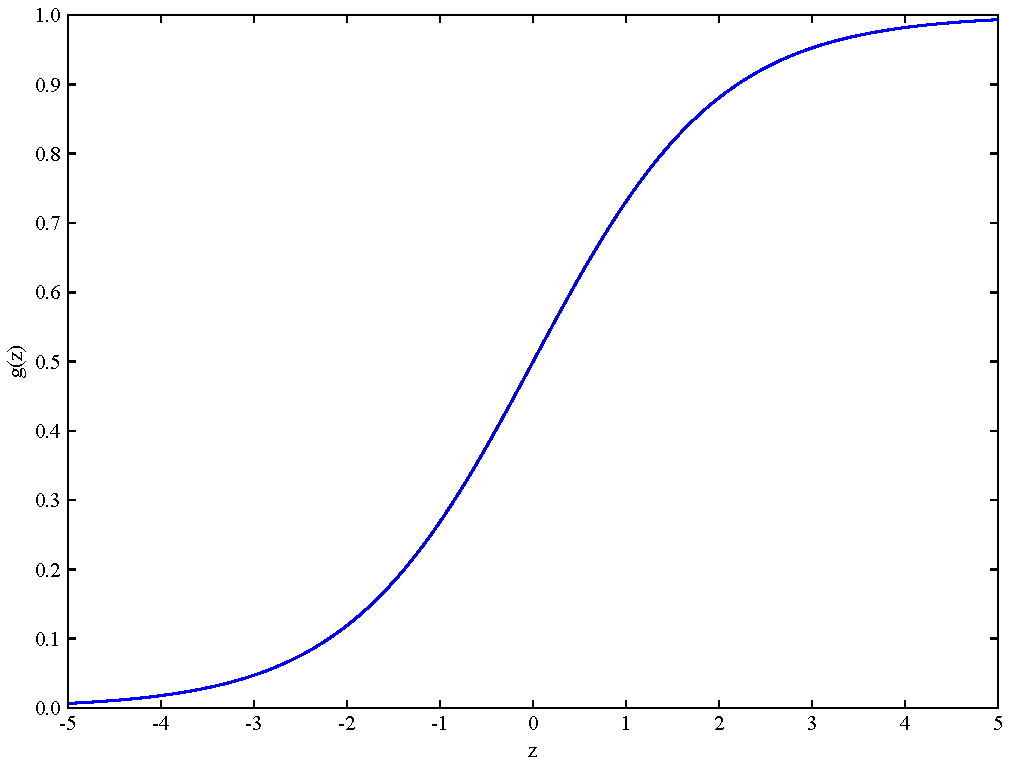
\includegraphics[width=0.5\linewidth]{figs/sigmoid.pdf}
    \label{fig:sigmoid}
\end{figure}

注意到 $g(z)$ 在 $z \to \infty$ 时趋于 1,在 $z \to -\infty$ 时趋于 0。此外,$g(z)$,因此 $h(x)$,始终介于 0 和 1 之间。和之前一样,这里约定 $x_0 = 1$,从而有 $\theta^T x = \theta_0 + \sum_{j=1}^d \theta_j x_j$。

现在先将 $g$ 的形式视为一个已知条件。其他从 0 平滑增加到 1 的函数也可以使用,但出于一些原因(稍后讨论广义线性模型(GLMs)和生成学习算法时会看到),选择 sigmoid 函数是相当自然的。在进一步展开之前,这里给出 sigmoid 函数导数的一个有用性质,记为 $g'$:
\[
    \begin{aligned}
        g'(z) &= \frac{d}{dz} \frac{1}{1+e^{-z}} \\ 
        &= \frac{1}{(1+e^{-z})^2} (e^{-z}) \\ 
        &= \frac{1}{1+e^{-z}} \cdot \left(1 - \frac{1}{1+e^{-z}}\right) \\ 
        &= g(z)(1 - g(z)).
    \end{aligned}
\]

那么,给定这样的逻辑回归模型,我们如何为其拟合 $\theta$ 呢?参照我们之前所见,最小二乘回归在一定假设下可以作为最大似然估计的一种形式。因此,我们也将为分类模型设定一组概率假设,然后通过最大似然估计的方式来拟合参数。

假设
\[
    \begin{aligned}
        P(y=1 \mid x; \theta) &= h_\theta(x) \\
        P(y=0 \mid x; \theta) &= 1 - h_\theta(x)
    \end{aligned}
\]
注意到上述两个概率表达式可以合并为一个更紧凑的形式
\[
    p(y \mid x; \theta) = (h_\theta(x))^y (1 - h_\theta(x))^{1-y}
\]
假设 $n$ 个训练样本是独立生成的,那么参数的似然可以写成
\[
    \begin{aligned}
        L(\theta) &= p(\vec{y} \mid X; \theta) \\ 
        &= \prod_{i=1}^n p(y^{(i)} \mid x^{(i)}; \theta) \\ 
        &= \prod_{i=1}^n (h_\theta(x^{(i)}))^{y^{(i)}} (1 - h_\theta(x^{(i)}))^{1-y^{(i)}}
    \end{aligned}
\]
和之前一样,最大化对数似然会更容易推导:
\begin{equation}
    \ell(\theta) = \log L(\theta) = \sum_{i=1}^n y^{(i)} \log h(x^{(i)}) + (1 - y^{(i)}) \log(1 - h(x^{(i)}))
    \label{eq:logistic_log_likelihood}
\end{equation}

那么,如何最大化这个似然函数呢呢?类似于线性回归的推导过程,我们可以采用梯度上升法。以向量形式表示,参数的更新规则为 $\theta := \theta + \alpha \nabla_\theta \ell(\theta)$。(注意更新公式中的正号,因为现在是在最大化函数,而不是最小化函数。)接下来,我们将从一个训练样本 $(x, y)$ 出发,推导随机梯度上升规则的导数:

\begin{align}
    \frac{\partial}{\partial \theta_j} \ell(\theta) &= \left(y \frac{1}{g(\theta^T x)} - (1-y) \frac{1}{1-g(\theta^T x)}\right) \frac{\partial}{\partial \theta_j} g(\theta^T x) \notag\\ 
    &= \left(y \frac{1}{g(\theta^T x)} - (1-y) \frac{1}{1-g(\theta^T x)}\right) g(\theta^T x)(1-g(\theta^T x)) \frac{\partial}{\partial \theta_j} \theta^T x \notag\\ 
    &= (y(1-g(\theta^T x)) - (1-y)g(\theta^T x)) x_j \notag\\
    &= (y - g(\theta^T x)) x_j \label{eq:partial_loss_theta}
\end{align}

上面的推导利用了 $g'(z) = g(z)(1-g(z))$ 这一点。这给出了随机梯度上升规则:
\[
    \theta_j := \theta_j + \alpha (y^{(i)} - h_\theta(x^{(i)})) x_j^{(i)}
\]
如果将推导出的逻辑回归更新规则与最小均方更新规则进行比较,会发现它们在形式上是相同的;但这并不是同一个算法,因为这里的 $h_\theta(x^{(i)})$ 是 $\theta^T x^{(i)}$ 的非线性函数。尽管如此,对于一个截然不同的算法和学习问题,却得到了相同的更新规则,这确实有些令人惊讶。这仅仅是巧合吗?抑或是背后存在更深层的原因?我们将在讨论广义线性模型(GLM)时解答这个问题。

\begin{remark}\label{remark:2.1.1}
    同一个损失函数的另一种表示方式也很有用,特别是在第 \ref{sec:7.1} 节研究非线性模型时。
\end{remark}
\noindent 设逻辑损失函数 $\ell_{\text{logistic}}: \mathbb{R} \times \{0, 1\} \to \mathbb{R}_{\ge 0}$ 定义为
\begin{equation}
    \ell_{\text{logistic}}(t, y) \triangleq y \log(1 + \exp(-t)) + (1 - y) \log(1 + \exp(t)).
\end{equation}
通过代入 $h_\theta(x) = 1/(1 + e^{-\theta^T x})$,可以验证负对数似然(方程 \eqref{eq:logistic_log_likelihood} 中 $\ell(\theta)$ 的负值)可以改写为
\begin{equation}
    -\ell(\theta) = \ell_{\text{logistic}}(\theta^T x, y).
\end{equation}
通常 $\theta^T x$ 或 $t$ 称为 \textit{logit}。稍作运算可得
\begin{align}
    \frac{\partial \ell_{\text{logistic}}(t, y)}{\partial t} &= y \frac{-\exp(-t)}{1 + \exp(-t)} + (1 - y) \frac{1}{1 + \exp(-t)} \\ 
    &= \frac{1}{1 + \exp(-t)} - y. \label{eq:2.6}
\end{align}
然后,使用链式法则,得到
\begin{align}
    \frac{\partial}{\partial \theta_j} \ell(\theta) &= - \frac{\partial \ell_{\text{logistic}}(t, y)}{\partial t} \cdot \frac{\partial t}{\partial \theta_j} \\ 
    &= (y-1/(1+\exp(-t))) \cdot x_j = (y - h_\theta(x)) x_j, 
\end{align}
这与方程 \eqref{eq:partial_loss_theta} 的推导是一致的。在第 \ref{sec:7.1} 节中,会看到这种观点可以扩展到非线性模型。

\section{离题:感知器学习算法}

现在,我们将简要讨论一个具有历史意义的算法,该算法在后续讨论学习理论时也将再次被提及。考虑对逻辑回归方法进行修改,“强制”其输出值为 0 或 1。为此,一个自然而然的想法是将函数 $g$ 的定义改为阈值函数:
\[
    g(z) = 
    \begin{cases} 
        1 & \text{若 } z \ge 0 \\
        0 & \text{若 } z < 0 
    \end{cases}
\]
如果像之前一样令 $h_\theta(x) = g(\theta^T x)$,但使用上述修改后的 $g$ 定义,并且使用更新规则
\[
    \theta_j := \theta_j + \alpha (y^{(i)} - h_\theta(x^{(i)})) x_j^{(i)}.
\]
那么就得到了\textbf{感知机学习算法 (perceptron learning algorithm)}。

在 20 世纪 60 年代,有人认为“感知机”是脑中单个神经元如何工作的一个粗略模型。考虑到该算法的简单性,在讨论学习理论时,它也将为分析提供一个起点。然而,请注意,尽管感知机看起来与其他讨论过的算法相似,但它实际上与逻辑回归和最小二乘线性回归是完全不同类型的算法;特别是,很难从概率角度解释感知机的预测结果,或者将感知机推导为最大似然估计算法。


\section{多类别分类}\label{sec:2.3}

考虑一个分类问题,其中响应变量 $y$ 可以取 $k$ 个值中的任意一个,即 $y \in \{1, 2, \dots, k\}$。例如,除了将电子邮件分为垃圾邮件或非垃圾邮件这两类(这是一个二元分类问题),也可能希望将其分为三类,例如垃圾邮件、个人邮件和工作相关邮件。标签/响应变量仍然是离散的,但现在可以取超过两个值。因此,将它建模为服从多项分布。

在这种情况下,$p(y \mid x; \theta)$ 是关于 $k$ 个可能的离散结果的分布,因此是多项分布。回想一下,多项分布涉及 $k$ 个数 $\phi_1, \dots, \phi_k$,它们指定了每个结果的概率。注意,这些数必须满足 $\sum_{i=1}^k \phi_i = 1$。将设计一个参数化模型,该模型输出满足此约束的 $\phi_1, \dots, \phi_k$,给定输入 $x$。

引入 $k$ 组参数 $\theta_1, \dots, \theta_k$,每组参数都是 $\mathbb{R}^d$ 中的一个向量。直观地,希望使用 $\theta_1^T x, \dots, \theta_k^T x$ 来表示$\phi_1, \dots, \phi_k$,即概率 $P(y = 1 \mid x; \theta), \dots, P(y = k \mid x; \theta)$。然而,这种直接方法存在两个问题。首先,$\theta_j^T x$ 不一定在 $[0, 1]$ 范围内。其次,$\theta_j^T x$ 的总和不一定为 1。因此,将使用 softmax 函数将 $(\theta_1^T x, \dots, \theta_k^T x)$ 转换为一个非负且总和为 1 的概率向量。

定义函数 $\text{softmax}: \mathbb{R}^k \to \mathbb{R}^k$ 如下:
\begin{equation}
    \text{softmax}(t_1, \dots, t_k) = 
    \begin{bmatrix} 
        \frac{\exp(t_1)}{\sum_{j=1}^k \exp(t_j)} \\
        \vdots \\
        \frac{\exp(t_k)}{\sum_{j=1}^k \exp(t_j)}
    \end{bmatrix}.
\end{equation}
softmax 函数的输入,即这里的向量 $t$,通常被称为 \textit{logits}。注意,根据定义,softmax 函数的输出始终是一个概率向量,其分量非负且总和为 1。

令 $(t_1, \dots, t_k) = (\theta_1^T x, \dots, \theta_k^T x)$。将 softmax 函数应用于 $(t_1, \dots, t_k)$,并将输出用作概率 $P(y = 1 \mid x; \theta), \dots, P(y = k \mid x; \theta)$。得到以下概率模型:
\begin{equation}
    \begin{bmatrix} 
        P(y = 1 \mid x; \theta) \\
        \vdots& \\
        P(y = k \mid x; \theta)
    \end{bmatrix} =
    \text{softmax}(t_1, \dots, t_k) = 
    \begin{bmatrix} 
    &\frac{\exp(\theta_1^T x)}{\sum_{j=1}^k \exp(\theta_j^T x)}& \\
    &\vdots& \\
    &\frac{\exp(\theta_k^T x)}{\sum_{j=1}^k \exp(\theta_j^T x)}&
    \end{bmatrix}.
\end{equation}
为了符号上的方便,令 $\phi_i = \frac{\exp(t_i)}{\sum_{j=1}^k \exp(t_j)}$。更简洁地,上面的方程可以写成:
\begin{equation}
    P(y = i \mid x; \theta) = \phi_i = \frac{\exp(t_i)}{\sum_{j=1}^k \exp(t_j)} = \frac{\exp(\theta_i^T x)}{\sum_{j=1}^k \exp(\theta_j^T x)}.
\end{equation}
接下来,计算单个样本 $(x, y)$ 的负对数似然。
\begin{equation}
    -\log p(y \mid x, \theta) = -\log\left(\frac{\exp(t_y)}{\sum_{j=1}^k \exp(t_j)}\right) = -\log\left(\frac{\exp(\theta_y^T x)}{\sum_{j=1}^k \exp(\theta_j^T x)}\right).
\end{equation}
因此,损失函数,即训练数据的负对数似然,由下式给出:
\begin{equation}
    \ell(\theta) = \sum_{i=1}^n -\log\left(\frac{\exp(\theta_{y^{(i)}}^T x^{(i)})}{\sum_{j=1}^k \exp(\theta_j^T x^{(i)})}\right).
    \label{eq:multiclass_loss}
\end{equation}
定义交叉熵损失 $\ell_{\text{ce}}: \mathbb{R}^k \times \{1, \dots, k\} \to \mathbb{R}_{\ge 0}$ 是很方便的,它将上述复杂的方程模块化为:\footnote{这里命名存在一些歧义。有些人将交叉熵损失定义为将概率向量(在本讲义中用 $\phi$ 表示)和标签 $y$ 映射到实数的函数,并将本讲义中的交叉熵损失称为 softmax-交叉熵损失。本讲义选择当前的命名约定是因为它与大多数现代深度学习库(如 PyTorch 和 Jax)的命名一致。}
\begin{equation}
    \ell_{\text{ce}}((t_1, \dots, t_k), y) = -\log \left( \frac{\exp(t_y)}{\sum_{j=1}^k \exp(t_j)} \right).
\end{equation}
使用此记号,方程 \eqref{eq:multiclass_loss} 可以简写为:
\begin{equation}
    \ell(\theta) = \sum_{i=1}^n \ell_{\text{ce}}((\theta_1^\top x^{(i)}, \dots, \theta_k^\top x^{(i)}), y^{(i)}).
\end{equation}
此外,交叉熵损失的梯度也很便于推导。令 $t = (t_1, \dots, t_k)$,并回顾 $\phi_i = \frac{\exp(t_i)}{\sum_{j=1}^k \exp(t_j)}$。可以推导出:
\begin{equation}
    \frac{\partial \ell_{\text{ce}}(t, y)}{\partial t_i} = \phi_i - {1}\{y=i\},
\end{equation}
其中 ${1}\{\cdot\}$ 是指示函数,即当 $y=i$ 时 ${1}\{y=i\} = 1$,当 $y \ne i$ 时 $\{y=i\} = 0$。向量化形式如下,这对于第 \ref{chapter:7} 章将很有用:
\begin{equation}
    \frac{\partial \ell_{\text{ce}}(t, y)}{\partial t} = \phi - e_y,\label{eq:2.17}
\end{equation}
其中 $e_s \in \mathbb{R}^k$ 是第 $s$ 个标准基向量(其中第 $s$ 个分量是 1,其余所有分量都是零)。使用链式法则,有:
\begin{equation}
    \frac{\partial \ell_{\text{ce}}((\theta_1^\top x, \dots, \theta_k^\top x), y)}{\partial \theta_i} = \frac{\partial \ell(t, y)}{\partial t_i} \frac{\partial t_i}{\partial \theta_i} = (\phi_i - {1}\{y=i\}) \cdot x.
\end{equation}
因此,损失函数关于参数 $\theta_i$ 的梯度为:
\begin{equation}
    \frac{\partial \ell(\theta)}{\partial \theta_i} = \sum_{j=1}^n (\phi_i^{(j)} - {1}\{y^{(j)}=i\}) \cdot x^{(j)},
\end{equation}
其中 $\phi_i^{(j)} = \frac{\exp(\theta_i^\top x^{(j)})}{\sum_{s=1}^k \exp(\theta_s^\top x^{(j)})}$ 是模型预测样本 $x^{(j)}$ 属于类别 $i$ 的概率。利用上述梯度,可以使用(随机)梯度下降来最小化损失函数 $\ell(\theta)$。

\section{最大化 \texorpdfstring{$\ell(\theta)$}{l(theta)} 的另一种算法}

回到以 sigmoid 为 $g(z)$ 函数的逻辑回归,现在讨论一种不同的最大化 $\ell(\theta)$ 的算法。

首先,考虑牛顿法用于寻找函数零点。具体来说,假设有一个函数 $f: \mathbb{R} \to \mathbb{R}$,并且希望找到一个 $\theta$ 值使得 $f(\theta) = 0$。这里 $\theta \in \mathbb{R}$ 是一个实数。牛顿法执行以下更新:
\[
    \theta := \theta - \frac{f(\theta)}{f'(\theta)}.
\]
这种方法有一种自然的解释:将函数 $f$ 通过其在当前猜测值 $\theta$ 处的切线进行近似,然后求解该切线等于零的点,并将该点作为 $\theta$ 的下一个猜测值。

以下是牛顿法实际应用的图示:

\begin{figure}[H]
  \centering
  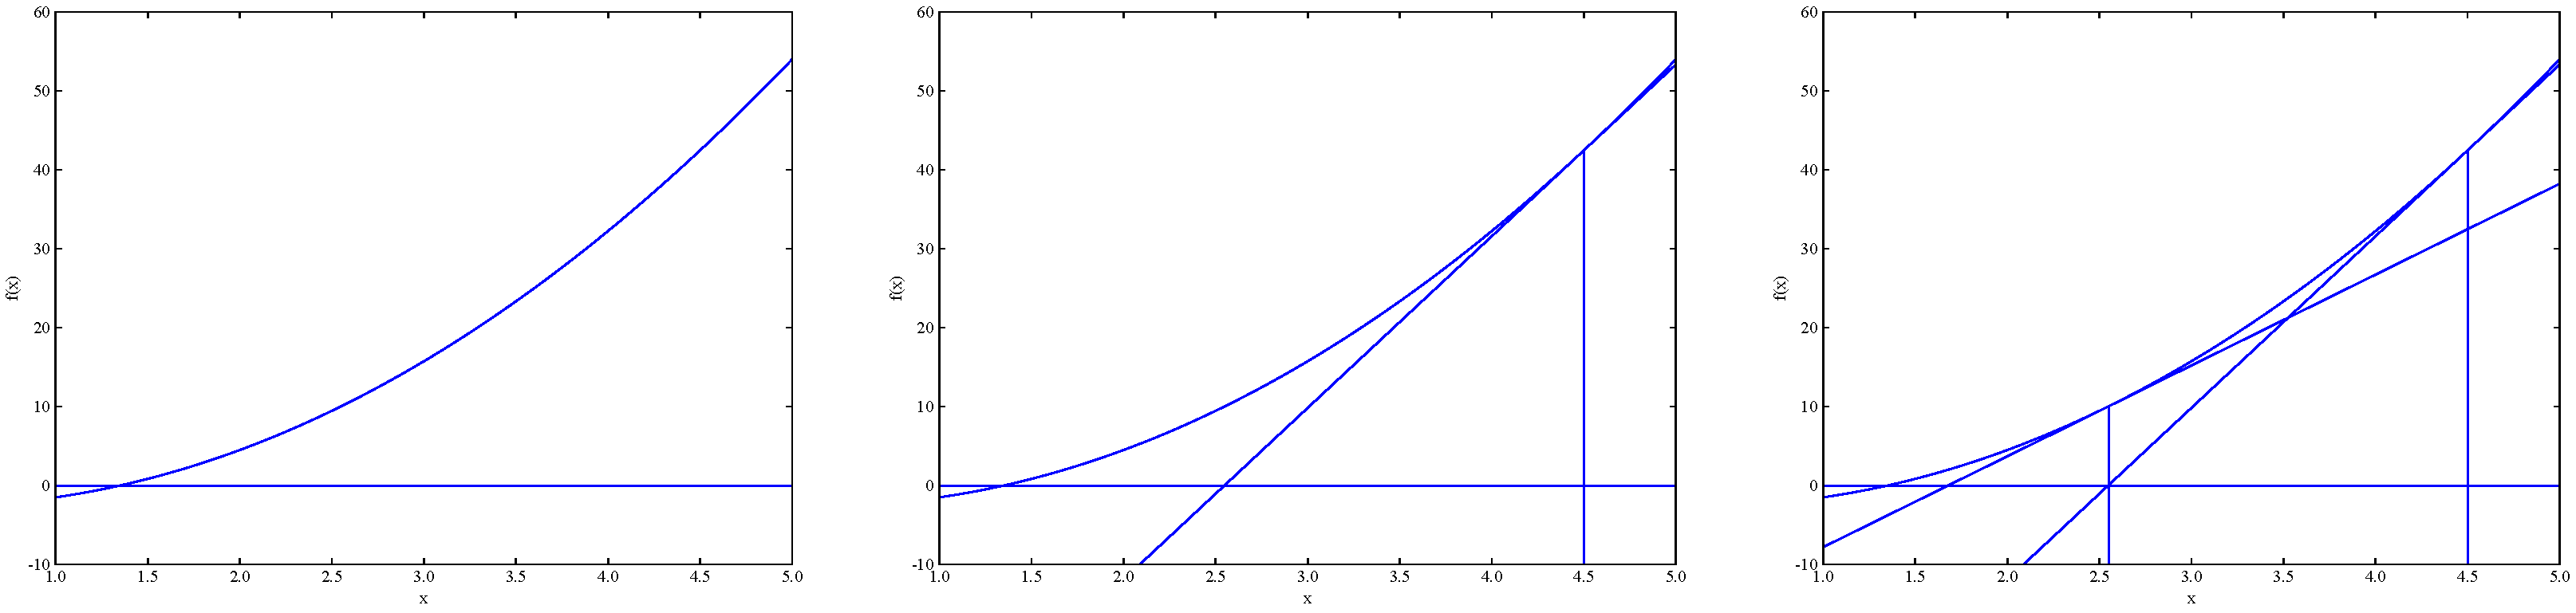
\includegraphics[width=0.93\linewidth]{figs/newton_iteration.pdf}
\end{figure}

\setcounter{footnote}{0}
\renewcommand{\thefootnote}{\fnsymbol{footnote}}
在最左边的图中,可以看到函数 $f$ 与直线 $y=0$。尝试找到一个 $\theta$ 使得 $f(\theta)=0$;实现这一点的 $\theta$ 值大约是 1.3。假设初始化的算法的 $\theta$ 值为 4.5。然后牛顿法拟合一条在 $\theta=4.5$ 处与 $f$ 相切的直线,并求解该直线等于 0 的点(中间图)。这给出了 $\theta$ 的下一个猜测值,大约是 2.6。最右边的图显示了再进行一次迭代的结果,更新后的 $\theta$ 大约是 1.6。再经过几次迭代后,将迅速接近 $\theta = 1.3$。\footnote{译者注:由于不知道原书所用函数的解析形式,这里译者画的图与原图稍有偏差,$\theta$的猜测值也稍有变化。}
\setcounter{footnote}{1}
\renewcommand{\thefootnote}{\arabic{footnote}}

牛顿法提供了一种求解 $f(\theta)=0$ 的方法。如果希望最大化某个函数 $\ell$ 呢? $\ell$ 的最大值对应于其一阶导数 $\ell'(\theta)$ 为零的点。因此,令 $f(\theta) = \ell'(\theta)$,可以使用相同的算法来最大化 $\ell$,并得到更新规则:
\[
    \theta := \theta - \frac{\ell'(\theta)}{\ell''(\theta)}.
\]
(思考题:如果希望使用牛顿法来最小化而不是最大化一个函数,这会如何改变?)

最后,在逻辑回归中,$\theta$ 是向量,因此需要将牛顿法推广到此情况。牛顿法在此多维设置中的推广(也称为牛顿-拉普森法)由下式给出
\[
    \theta := \theta - H^{-1} \nabla_\theta \ell(\theta).
\]
这里,$\nabla_\theta \ell(\theta)$ 是 $\ell(\theta)$ 对 $\theta_i$ 的偏导数向量,而 $H$ 是一个 $d \times d$ 矩阵(实际上,如果包含截距项,则是 $(d+1) \times (d+1)$ 矩阵),称为\textbf{Hessian} 矩阵,其元素由下式给出
\[
    H_{ij} = \frac{\partial^2 \ell(\theta)}{\partial \theta_i \partial \theta_j}.
\]
牛顿法通常比(批量)梯度下降收敛更快,并且需要更少的迭代次数即可非常接近最小值。然而,牛顿法迭代一次比梯度下降迭代一次更昂贵,因为它需要找到一个 $d \times d$ 的 Hessian 矩阵并求逆;但只要 $d$ 不太大,通常总体上会快得多。当牛顿法应用于最大化逻辑回归对数似然函数 $\ell(\theta)$ 时,所得方法也称为 \textbf{Fisher scoring}。